
\pdfminorversion=4
\documentclass[xcolor=dvipsnames,fontsize=8pt]{beamer}
\usepackage{tabls}
\usepackage{verbatim}
\usepackage{graphicx}
%\usepackage{animate}
\usepackage{xcolor}

%tikz stuff
\usepackage{tikz}
\usetikzlibrary{shapes.geometric, arrows}
\tikzstyle{startstop} = [rectangle, rounded corners, minimum width=2cm, text
    width=1.8cm, minimum height=1cm,text centered, text=white,draw=black, fill=Gray!140]
\tikzstyle{io} = [trapezium, trapezium left angle=70, trapezium right angle=110,
minimum width=0.5cm, minimum height=1cm, text centered, draw=black,
fill=blue!20!Gray!90!,text=white]
\tikzstyle{process} = [rectangle, minimum width=2cm, minimum height=1cm, text
centered, text width=2cm, draw=black, text=white,fill=Gray!140!blue!70!white]
\tikzstyle{decision} = [diamond, minimum width=3cm, minimum height=1cm, text
centered, draw=black, fill=Gray!,text=white]
\tikzstyle{arrow} = [thick,line width=0.6mm,->,>=stealth]
\tikzstyle{arrow1} = [dashed,->,>=stealth]
\setbeamertemplate{navigation symbols}{}
\setbeamertemplate{footline}[frame number]

%\definecolor{myblue}{rgb}{0.7, 0.7, 60.0}
\definecolor{mylightblue}{rgb}{1,1,1}
\newcommand*{\boxedcolor}{blue}
\newcommand{\bracket}[1]{\left[ #1 \right]}
\newcommand{\bracet}[1]{\left\{ #1 \right\}}
\newcommand{\fn}[1]{\left( #1 \right)}
\newcommand{\ave}[1]{\left\langle #1 \right\rangle}
\newcommand{\norm}[1]{\Arrowvert #1 \Arrowvert}
\newcommand{\abs}[1]{\arrowvert #1 \arrowvert}
\newcommand{\BU}[0]{\ensuremath{\mathbf{U}}}
\newcommand{\BY}[0]{\ensuremath{\mathbf{Y}}}
\newcommand{\BQ}[0]{\ensuremath{\mathbf{Q}}}
\newcommand{\E}{\mathcal{E}}
\newcommand{\F}{\mathcal{F}}

\makeatletter
\renewcommand{\boxed}[1]{\textcolor{\boxedcolor}{%
  \fbox{\normalcolor\m@th$\displaystyle#1$}}}
\makeatother
\usepackage{hyperref}

\newcommand{\backupbegin}{
   \newcounter{framenumberappendix}
   \setcounter{framenumberappendix}{\value{framenumber}}
}
\newcommand{\backupend}{
   \addtocounter{framenumberappendix}{-\value{framenumber}}
   \addtocounter{framenumber}{\value{framenumberappendix}} 
}
\renewcommand{\u}[1]{\underline{#1}}

\newcommand{\iso}[2]{${}^{{#2}}${#1} }
\newcommand{\nubar}[0]{$\overline{\nu}$ }
\newcommand{\keff}[0]{\ensuremath{{k}_{\textsf{eff}}} }
\newcommand{\expect}[1]{E[#1] }
\newcommand{\colg}[1]{{\color{ForestGreen} #1}}
\newcommand{\coly}[1]{{\color{yellow} #1}}
\newcommand{\colb}[1]{{\color{blue} #1}}
\newcommand{\colr}[1]{{\color{red} #1}}
\usepackage{amsfonts}
\newlength{\wideitemsep}
\setlength{\wideitemsep}{8pt}
%\addtolength{\wideitemsep}{5pt}
\let\olditem\item
\renewcommand{\item}{\setlength{\itemsep}{\wideitemsep}\olditem}

\newcommand{\N}{\mathbb{N}}
\newcommand{\Z}{\mathbb{Z}}
\newcommand{\deriv}[2]{\frac{\mathrm{d} #1}{\mathrm{d} #2}}
\newcommand{\pderiv}[2]{\frac{\partial #1}{\partial #2}}
\newcommand{\bx}{\mathbf{X}}
\newcommand{\ba}{\mathbf{A}}
\newcommand{\by}{\mathbf{Y}}
\newcommand{\bj}{\mathbf{J}}
\newcommand{\bs}{\mathbf{s}}
\newcommand{\B}[1]{\ensuremath{\mathbf{#1}}}
\newcommand{\Dt}{\Delta t}
\newcommand{\Dx}{\Delta x}
\renewcommand{\d}{\mathsf{d}}
\newcommand{\mom}[1]{\langle #1 \rangle}
\newcommand{\xl}{{x_{i-1/2}}}
\newcommand{\xr}{{x_{i+1/2}}}
\newcommand{\il}{{i-1/2}}
\newcommand{\ir}{{i+1/2}}

\AtBeginSection[]
{
    \begin{frame}<beamer>
        \frametitle{Outline}
        \tableofcontents[currentsection]
    \end{frame}
}

\setbeamerfont{frametitle}{size=\Large}
\setbeamerfont{normal font}{size=\tiny}

\graphicspath{{figures/}}

\usepackage{verbatim}
\usepackage{comment}
\usepackage[]{datetime}
\usepackage{multirow}

\newcommand{\thedate}{\today}


\setlength{\tabcolsep}{1.05cm}
\geometry{paperwidth=140mm,paperheight=105mm}

%Aggie-themed
\pgfdeclareimage[height=0.1in]{TAMUlogo}{tamu_engineering.png}
\logo{\raisebox{-8pt}{\pgfuseimage{TAMUlogo}}}
\titlegraphic{\centering\begin{tabular}{c}

\includegraphics[height=0.18\textheight]{tamu_seal.png}\end{tabular}}
%Michigan-themed
%\pgfdeclareimage[height=0.1in]{UMlogo}{michigan_engineering.png}
%\logo{\raisebox{-8pt}{\pgfuseimage{UMlogo}}}
%\titlegraphic{
\includegraphics[height=0.2\textheight]{michigan_block_m.png}}


%%%%%%%%%%%%%%%%%%%%%%%%%%%%%%%%%%%%%%%%%%%%%%%%%%%%%%%%%%%%%%%
% Optional packages, used to show off certain tricks

\newlength \figwidth
\setlength \figwidth {0.5\textwidth}

\setlength{\leftmargin}{-2cm}
\setlength{\rightmargin}{-2cm}

%%%%%%%%%%%%%%%%%%%%%%%%%%%%%%%%%%%%%%%%%%%%%%%%%%%%%%%%%%%%%%%

\usepackage[english]{babel}
\usetheme{Frankfurt}

%Make it Aggie Maroon
\usecolortheme[RGB={80,0,0}]{structure}  
%Or Michigan Blue
%\usecolortheme[RGB={0,0,153}]{structure}  
%Or Michigan Maize
%\usecolortheme[RGB={255,204,0}]{structure}  

  % This will typeset only the frames (or slides) that have the given label ("current" in this case).

\title{Second-Order Discretization in Space and Time for Grey S$_2$-Radiation Hydrodynamics}
    \author{{\large Simon R. Bolding, Joshua E. Hansel, \& Jim E. Morel}}
\date{16 October 2015 \\ \vspace{0.05in} {CLASS seminar}}
\subject{}
%\institute{Los Alamos National Laboratory}

% \classificationlevel{SECRET/RD}
% \transmissible{}

%\reportnum{\textcolor{blue}{SAMPLE TEMPLATE ONLY \\ Contains NO Classified
%Information}}

%\dissableframenumber
\begin{document}

\begin{frame}
    \titlepage \vspace{-0.213in}
    \begin{center}
    \end{center}    
\end{frame}

\setlength{\tabcolsep}{6pt}

\begin{frame}
\frametitle{Outline}
\begin{minipage}{0.061\linewidth}
\hfill                      
\end{minipage}
\begin{minipage}{0.8\linewidth}
\tableofcontents[
hideothersubsections,
sectionstyle=show,
subsectionstyle=hide
]
\end{minipage}

\end{frame}


\section{Overview}
\subsection{}

\begin{frame}
    \frametitle{What is radiation hydrodynamics?}
    \begin{itemize}
        \item Thermal radiative transfer (TRT) coupled to material hydrodynamics
            \begin{itemize}
                \item Inertial confinement fusion (NIF) and astrophysics calculations
            \end{itemize}
    \end{itemize}
    \begin{figure}
    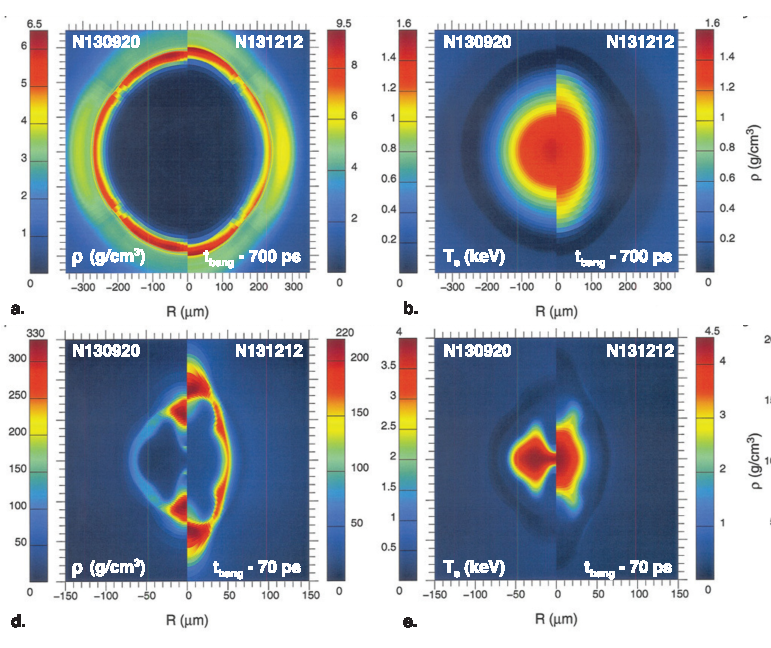
\includegraphics[width=0.6\textwidth,trim=0.1in 0.1in 0.0in 0.1in,clip]{nif.pdf}
    \caption{Comparison of HYDRA simulations for collapses of 2 NIF hohlraum designs, from Meezan et.
    al., 2015}
    \end{figure}
\end{frame}

\begin{frame}
    \frametitle{We have implemented and tested a 2$^{\textsf{nd}}$ order solution method}
        \begin{itemize}
            \item Previous work by Edwards and Morel for an algorithm that is second-order in
     \colb{space} and \colb{time}
            \item \textbf{Hydrodynamics} is solved with a MUSCL-Hancock method predictor-corrector
                in time
            \item \textbf{Radiation diffusion} is solved with linear discontinuous finite
                elements in space and a conservative form of TRBDF2 in time
            \item Resolves issues with mixing of implicit and explicit time
                    discretizations, as well as different spatial discretizations 
            \item Used approximate radiation hydrodynamics equations that produce the correct
        equilibrium diffusion limit solution to $\mathcal{O}(u/c)$
        \end{itemize}
        \begin{block}{We have extended the method to S$_2$ equations }
     \begin{itemize}
        \item S$_2$ allows for conservation of momentum
        \item Can be generalized to S$_n$ equations, but would also be well suited
            for a high-order low-order approach 
     \end{itemize}
     \end{block}
\end{frame}

\begin{frame}
    \frametitle{The non-relativistic radiation hydrodynamics equations}
    \begin{itemize}
        \item For hydro, we have the 1D Euler Equations with source terms from interaction and emission of \colb{radiation} (grey)
            \begin{equation}
                \boxed{
                    \pderiv{ }{t}\BU + \pderiv{ }{x}F(\BU) = \mathbf{Q(\BU)}}
            \end{equation}
            \begin{tabular}{ccc}
                $\BU = \begin{pmatrix} \rho \\ \rho u \\ E \end{pmatrix}$, 
                & $F(\BU) = \begin{pmatrix} \rho u \\ \rho u^2 + p \\ u\fn{E + p}
                \end{pmatrix}$, 
                & $Q(\BU) = \begin{pmatrix} 0 \\ \colb{Q_{\textsf{mom}}} \\
                    \colb{Q_{\textsf{erg}}}
                \end{pmatrix}$
            \end{tabular}
        \item The coupling terms are
            \begin{align*}
                \colb{Q_{\textsf{mom}}} = \frac{\sigma_t}{c} \F_0 , \quad & \quad
                \colb{Q_{\textsf{\textsf{erg}}}}=-\sigma_a
                    c \left( aT^4 - \E \right) + \frac{\sigma_t u}{c} \F_0
            \end{align*}
        \item There is an equation of state to relate internal energy $e$ and $T$
        \item The Euler equations are typically solved with explicit time discretizations that require a \colb{time step limit} (CFL)
    \end{itemize}
\end{frame}

\begin{frame}
    \frametitle{The $S_2$ equations for radiation hydrodynamics}
    \begin{itemize}
    \item The radiation transport equation contains source and loss terms from
        interaction with material
    \item To get S$_2$ equations, we collocate to $\mu=\pm\frac{1}{\sqrt{3}}$
        to get equations for half-range intensities $I^\pm$
        \begin{align*}
\frac{1}{c}\pderiv{I^+(x,t)}{t} + \frac{1}{\sqrt{3}}\pderiv{I^+}{x} + \sigma_t
I^+ &= 
\frac{\sigma_s}{4\pi} c\E + \frac{\sigma_a}{4\pi} acT^4  - \frac{\sigma_t u}{4\pi c}
\F_{0} +  
\frac{\sigma_t}{\sqrt{3}\pi}\E u,  \\
\frac{1}{c}\pderiv{I^-(x,t)}{t} - \frac{1}{\sqrt{3}}\pderiv{I^-}{x} + \sigma_t
I^+ &= 
\frac{\sigma_s}{4\pi} c\E + \frac{\sigma_a}{4\pi} acT^4  - \frac{\sigma_t u}{4\pi c}
\F_{0} -  
\frac{\sigma_t}{\sqrt{3}\pi}\E u, 
\end{align*} 
    \item with
        \begin{align*}
        \E = \frac{1}{c}2\pi\int_{-1}^1\!\! I(\mu)\; \d \mu, \quad & \quad \F =
        2\pi\int_{-1}^1\!\! \mu\, I(\mu) \; \d \mu, \quad & \quad   \F_0 = \F - \frac{4}{3}\E u
        \end{align*}
    \item These equations are solved using \colb{implicit} time discretizations
    \item Angular moments of the S$_2$ equations gives the radiation balance
        and momentum equations, with correct $-Q_{\textsf{erg}}$ and $-Q_{\textsf{mom}}$
\end{itemize}
\end{frame}

\begin{frame}
    \frametitle{Solution to the radiation hydrodynamics equations}
     \begin{itemize}
        \item Combining equations from last two slides gives full rad-hydro equations
        \item Operator splitting in time is used to separate the Euler equations 
            from thermal radiative transfer equations. 
            \begin{itemize}
                \item In our notation Euler equations will advect hydro variables
                    from $U$ to $U^*$, 
            \end{itemize}
        \item For hydrodynamics, we use a Eularian mesh where the mesh is fixed and mass flows between
            cells
        \item The radiation and internal energy have to be solved with a Newton's method due to
            non-linear emission term $\sigma_a a c T^4$
        \item An outer fixed point method is used to compute for comoving frame flux
            term $\F_0$, which is a function of $u$
        \item Want to conserve balance of total energy, momentum, and mass
     \end{itemize}
\end{frame}

\section{Solution to Euler Equations}

\begin{frame}
    \frametitle{The MUSCL Hancock method is second-order accurate in $x$ \& $t$}
    \begin{itemize}
        \item The MUSCL Hancock method uses \colb{slope-limited} reconstruction in
            space and \colb{explicit} predictor-corrector steps in time
    \begin{figure}[h]
        \centering
        \resizebox{0.64\textwidth}{!}{
        \input{slope_tilting.pdf_tex}
        }
    \end{figure}
    \item For the predictor step interior $F(\BU)$ is used on the faces.  For the
        corrector step, an \colb{approximate Riemann solver} is used for
        $F_{i\pm1/2}(\BU)$.  
    \item The time from $t_n$ to $t_{n+1}$ is
        \begin{itemize} 
            \item[] \u{ Step 1:}
        \begin{equation*}
            U_i^* = U_i^n - \frac{\Dt}{2\Dx}\left[F(\BU_{i,R}^n) - F(\BU_{i,L}^n)\right]
        \end{equation*}
    \item[] \u{ Step 2:}
        \begin{equation*}
            U^{N+1} = U^n - \frac{\Dt}{\Dx}\left[\colb{F(\BU_{i+1/2}^*) -
            F(\BU_{i-1/2}^*)}\right]
        \end{equation*}
        \end{itemize}
    \end{itemize}
\end{frame}

\section{Solution to TRT Equations}

\begin{frame}
    \frametitle{Time stepping for the radiation and total energy solves}
    \begin{itemize}
        \item  We use a combination of Crank-Nicholson (CN) and a modified
            version of  BDF2 
        \item The BDF2 step takes place over a second half time step, rather than the
            over the full time step.
        \item This is done to conserve total energy and momentum over the full time
            step, in conjuction with the two explicit hydro steps.
        \item As an example, consider $\frac{\d \BY}{\d t} = f(\BY)$. Our algorithm uses
            \begin{equation*}
                \frac{(\BY^{n+1/2} - \BY^n)}{\frac{\Dt}{2}} = \frac{1}{2}\left[f(\BY^{n+1/2}) + f(\BY^{n})\right]
            \end{equation*}
            \begin{equation*}
            \frac{(\BY^{n+1} - \BY^{n+1/2})}{\frac{\Dt}{2}} = \frac{2}{3}f(\BY^{n+1})
        + \frac{1}{6}f(\BY^{n+1/2})+ \frac{1}{6}f(\BY^{n})
            \end{equation*}
    \end{itemize}
\end{frame}

\begin{frame}
    \frametitle{Linear Discontinuous Galerkin Spatial Discreziation for TRT}
    \begin{itemize}
    \item Within a Newton step, the material energy equation can be eliminate, leaving the equations for the radiation as a fixed source problem
        \begin{equation}
            \pm\frac{1}{\sqrt{3}}
            \pderiv{I^\pm}{x} + {\hat\sigma_t} I^\pm  - \frac{\hat\sigma_sEc}{4\pi} = \hat Q
        \end{equation}
        where $\hat{\cdot}$ quantities depend on the time discretization and material energy linearization
    \item We use a lumped LDFE in space with \colb{upwinding} to define $I$ on faces
    \begin{figure}
    \begin{centering}
        \begin{tikzpicture}[scale=0.758, every node/.style={transform shape}]
            \draw (1.0,4.0) node[fill,circle,inner sep=0pt,minimum
            size=4.2pt] {};
            \filldraw[color=black, fill=white] (1,2.1250) circle (2.1pt);
            \draw [->] (1.6,4.25) -- (2.4,4.25) node[anchor=west] {$\mu$};
            \draw (1.0,0.4) -- (1.0,0.6) node[below, pos=0.4] {$x_{i-1/2}$};
            \draw (5.90,0.4) -- (5.90,0.6) node[below, pos=0.4] {$x_{i+1/2}$};
            \node at (4.6,3.70) {$I^+(x)$};
            \draw [thick] (1.0,0.5) -- (5.9,0.5) node[anchor=north west] {};
            \draw (1.0,2.125) -- (5.90,3.70);
            \draw [dashed] (5.90,0.5) -- (5.90,4);
            \draw [dashed] (1.0,0.5) -- (1.0,4);
        \end{tikzpicture}
    \end{centering}
    \end{figure}
    \item Fully discrete system is formed with spatial unknowns at the left and right edges of a cell. The system can be inverted directly for S$_2$
\end{itemize}
\end{frame}

\section{The algorithm}

\begin{frame}
    \frametitle{Non-linear iteration scheme for each implicit solve} 
    \begin{itemize}
        \item Herein ``non-linear solve'' refers to a simultaneous solve of the equations for S$_2$ equations, radiation momentum deposition, and new total material energy
        \item \colb{Algorithm}
    \begin{enumerate}
        \item Update material momentum from radiation deposition
        \item Using Newtons method, we eliminate the material energy equation and
            solve for a new $I^\pm$, and thus $\E$
        \item Update material internal energy equation based on new $\E$
    \end{enumerate}
        \item Energy and momentum updates use lagged $\F_{0}$
        \item \emph{Initial} numerical tests indicate the momentum update may be unstable if $E/\rho
            u^2$ or $u/c$ are too large
        \item We only conserve momentum to the tolerance of outer iteration
    \end{itemize}
\end{frame}

\begin{frame}
    \frametitle{Time stepping algorithm, \coly{first half} of time step}
    \begin{figure}[h]
        \centering
        \input{time_stepping.pdf_tex}
    \end{figure}
\end{frame}

\begin{frame}
    \frametitle{Time stepping algorithm, \coly{second half} of time step}
    \begin{figure}[h]
        \centering
        \input{time_stepping_2.pdf_tex}
    \end{figure}
\end{frame}

\begin{frame}
    \frametitle{Why all the steps?! This seems expensive\ldots}
    \begin{itemize}
        \item In a TRBDF2 scheme, we need a second order accurate estimate of solution
            at $t_{n+1/2}$ 
            \begin{equation*}
            \frac{(\BU^{n+1} - \BU^{n+1/2})}{\frac{\Dt}{2}} = \frac{2}{3}f(\BU^{n+1})
        + \colb{\frac{1}{6}f(\BU^{n+1/2})}+ \frac{1}{6}f(\BU^{n})
            \end{equation*}
        \item If we used a MH predictor to $t_{n+1/2}$, then the hydro variables
            would only be first order accurate
        \item The 4 nonlinear solves are not that bad\ldots The maximum allowable size of $\Dt$ based on CFL limit is
            now twice as big.  
        \item For the same total number of hydro steps, we do the same amount of work as a two step method, but are \colb{second order accurate}
    \end{itemize}
\end{frame}

\section{Results}
\subsection{}

\begin{frame}
    \frametitle{Method of Manufactured Solutions}
    \begin{itemize}
        \item Add effective source equation
        \item saem for radiation
        \item Adds in a mass term. blah blah
        \item Use same temporal discretization for sources, but quadruature for high
            accuracy spatial integration of sources 
        \item Can be automated relatively easily with \textbf{Sympy}
    \end{itemize}
\end{frame}

\begin{frame}
    \frametitle{Before and after of schock solution}
    \begin{itemize}
        \item Shock is a discontinuity in the solution
        \item 
    \end{itemize}

\end{frame}

\begin{frame}
\frametitle{Results}
\framesubtitle{Pure Hydrodynamics: Shock Tube Problem Solutions with van Leer
  Slope Limiter}

\begin{center}
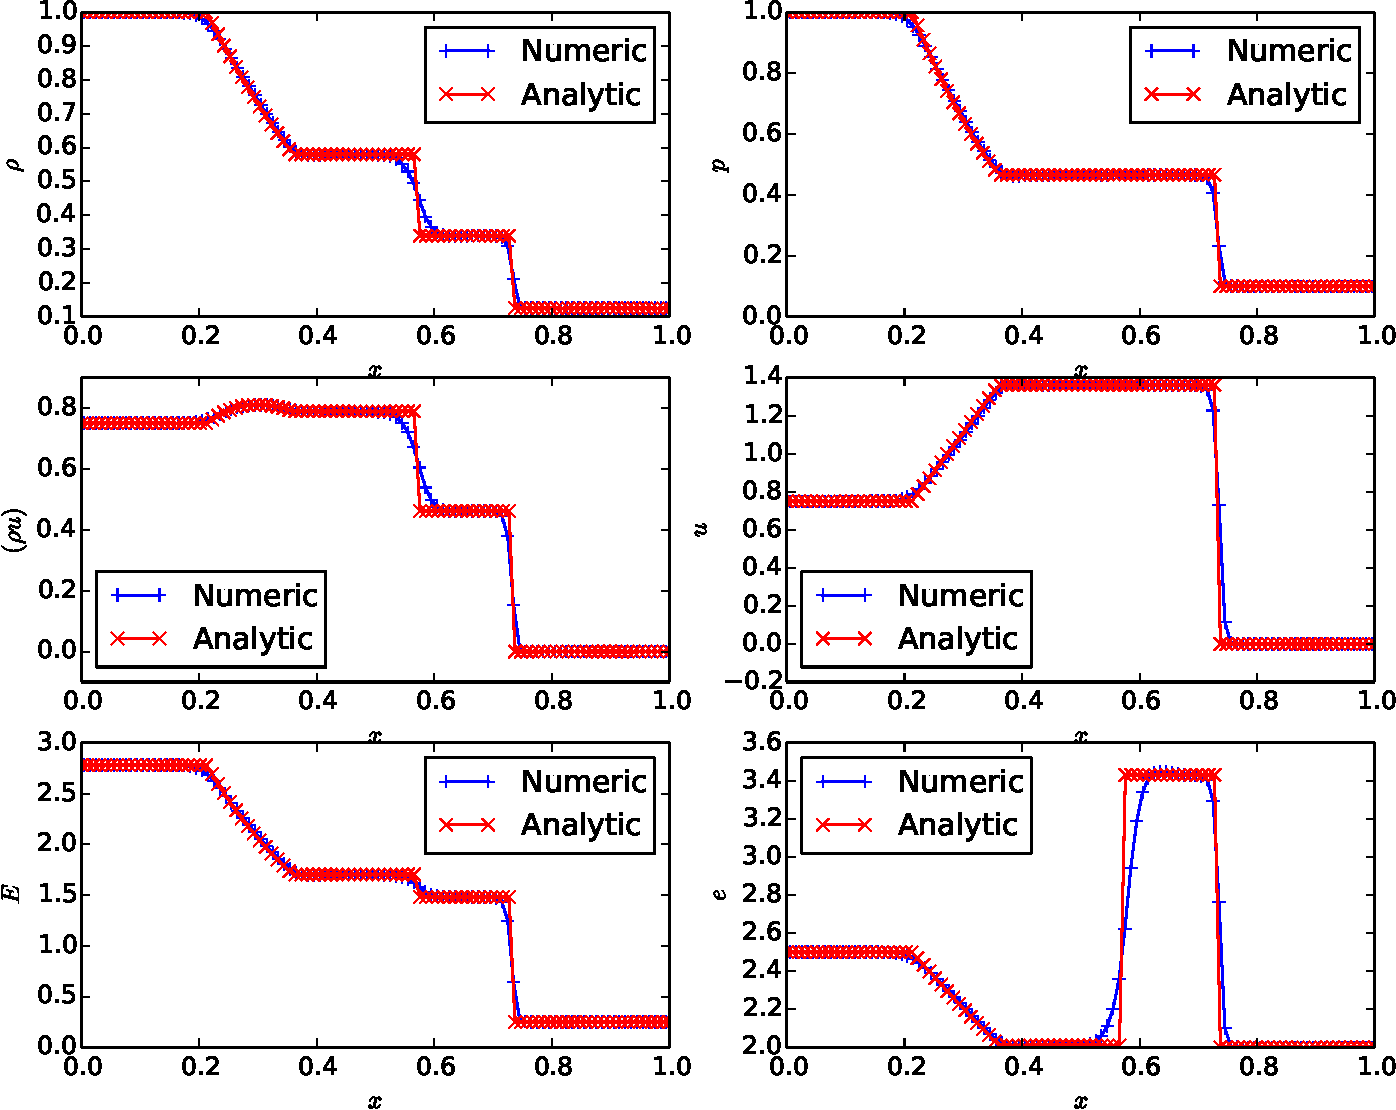
\includegraphics[width=0.9\textwidth]{./figures/shock_tube.pdf}
\end{center}
\end{frame}
%%%%%%%%%%%%%%%%%%%%%%%%%%%%%%%%%%%%%%%%%%%%%%%%%%%%%%%%%%%%%%%%%%%%%%%%%%%%%%%%%

\begin{frame}
\frametitle{Results}
\framesubtitle{Diffusion-Limit MMS Problem Solutions}

\begin{center}
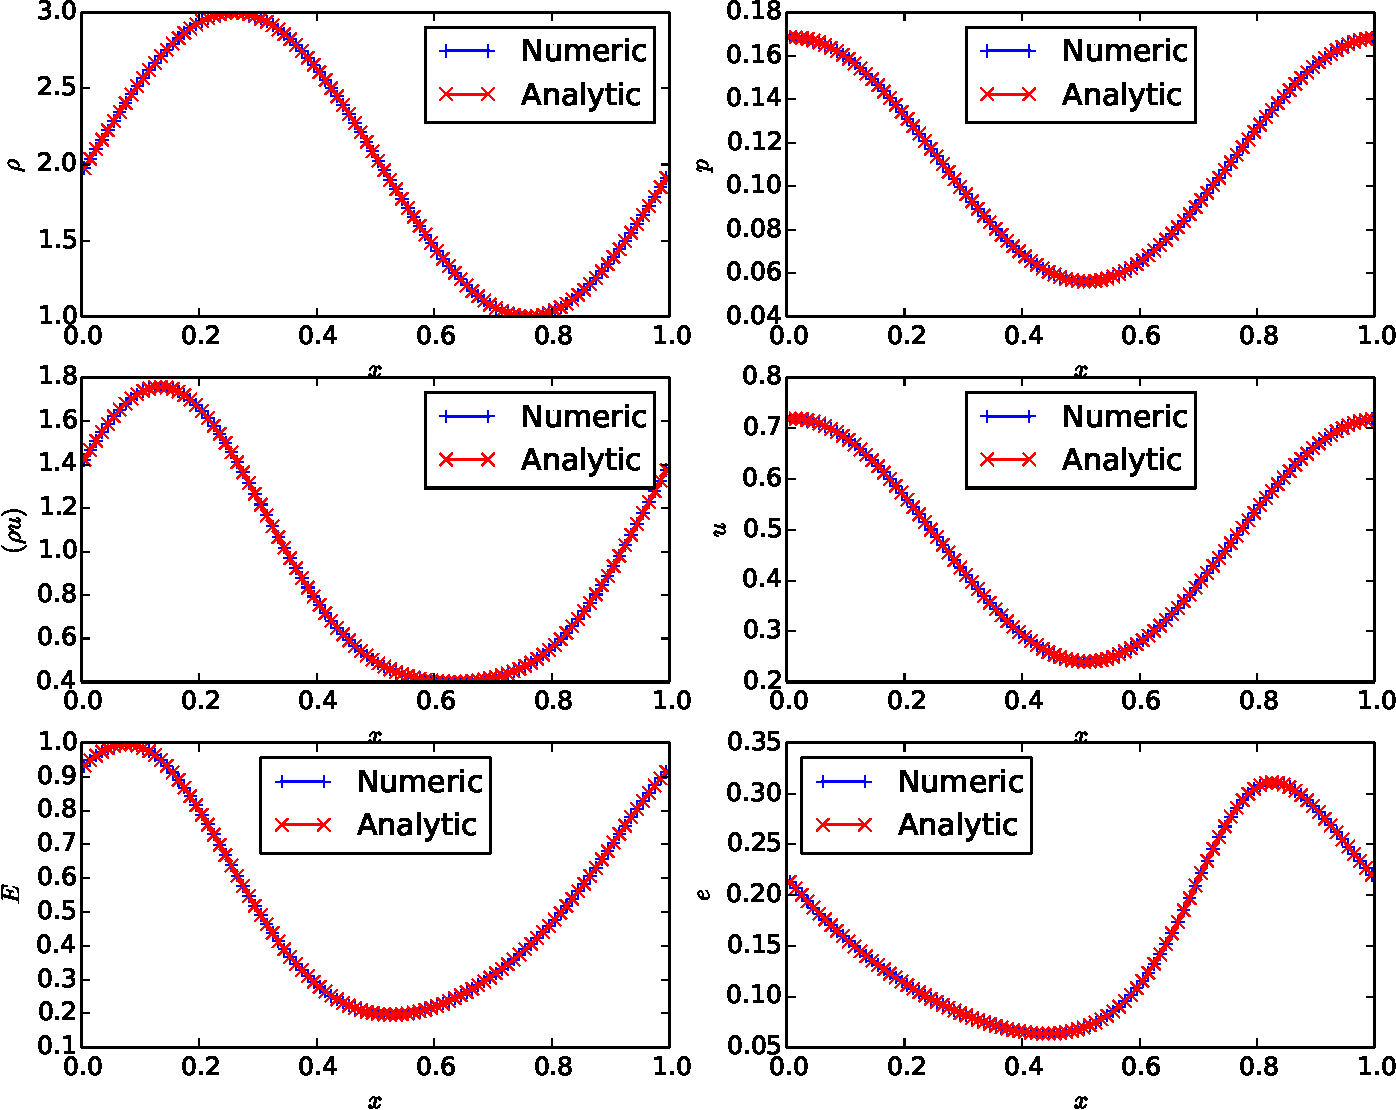
\includegraphics[width=0.9\textwidth]{./figures/MMS_solution.pdf}
\end{center}

\end{frame}
%%%%%%%%%%%%%%%%%%%%%%%%%%%%%%%%%%%%%%%%%%%%%%%%%%%%%%%%%%%%%%%%%%%%%%%%%%%%%%%%%
\begin{frame}
\frametitle{Results}
\framesubtitle{Convergence Rate for Diffusion-Limit MMS Problem}

\begin{center}
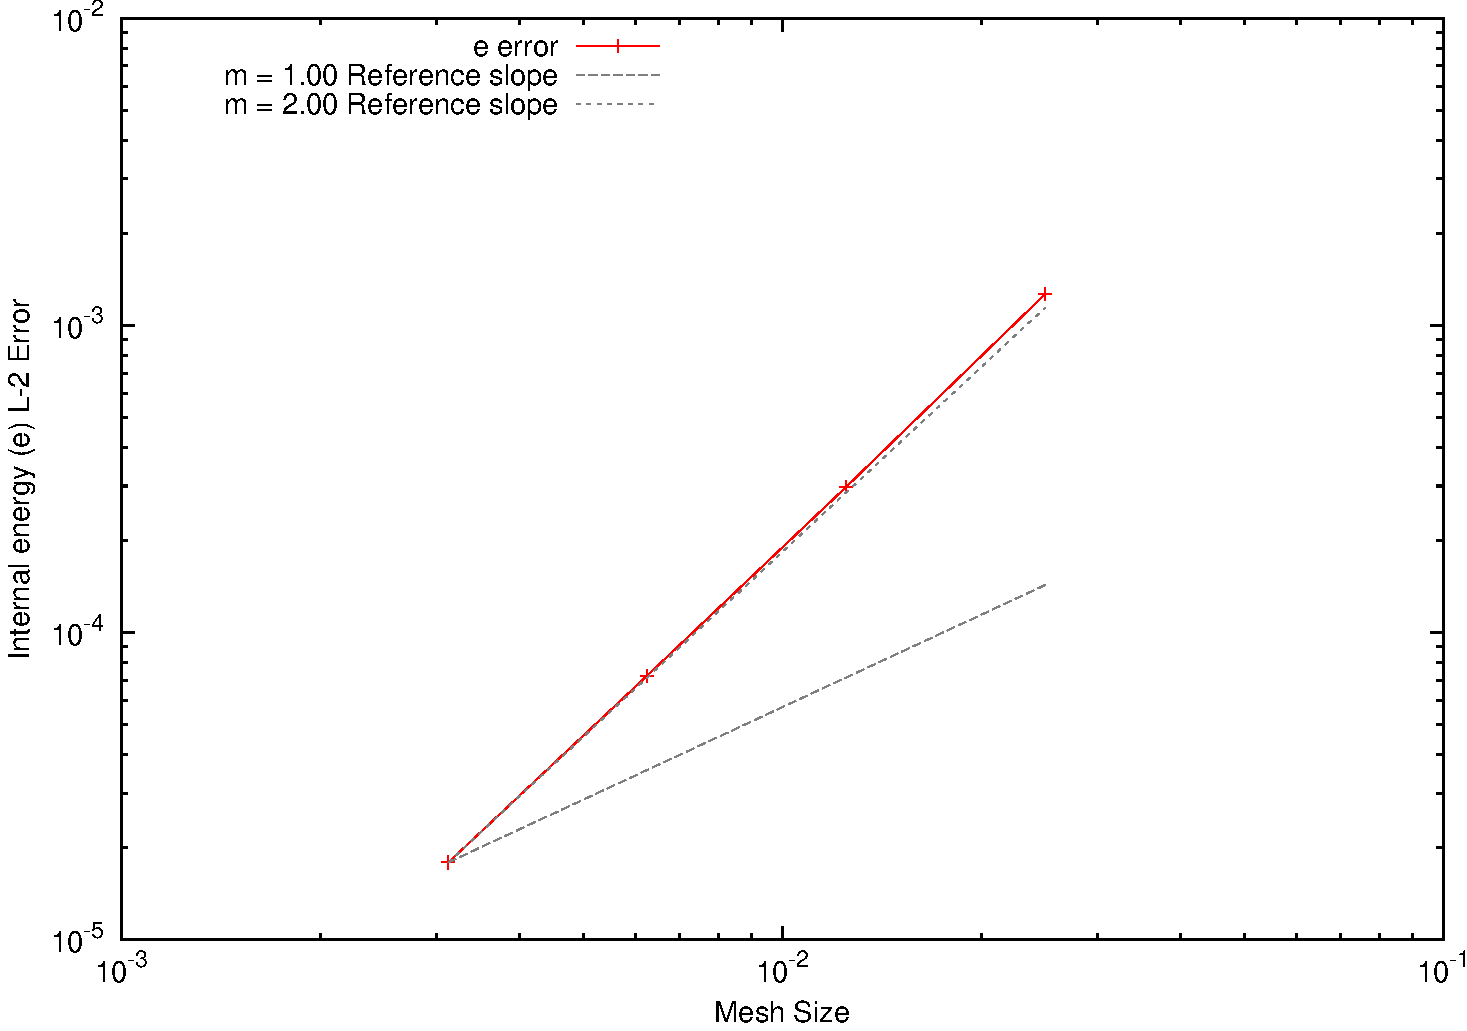
\includegraphics[width=0.9\textwidth]{./figures/MMS_convergence.pdf}
\end{center}

\end{frame}
%%%%%%%%%%%%%%%%%%%%%%%%%%%%%%%%%%%%%%%%%%%%%%%%%%%%%%%%%%%%%%%%%%%%%%%%%%%%%%%%%
\begin{frame}
\frametitle{Results}
\framesubtitle{Mach 2 Radiation-Hydrodynamics Shock}

\begin{center}
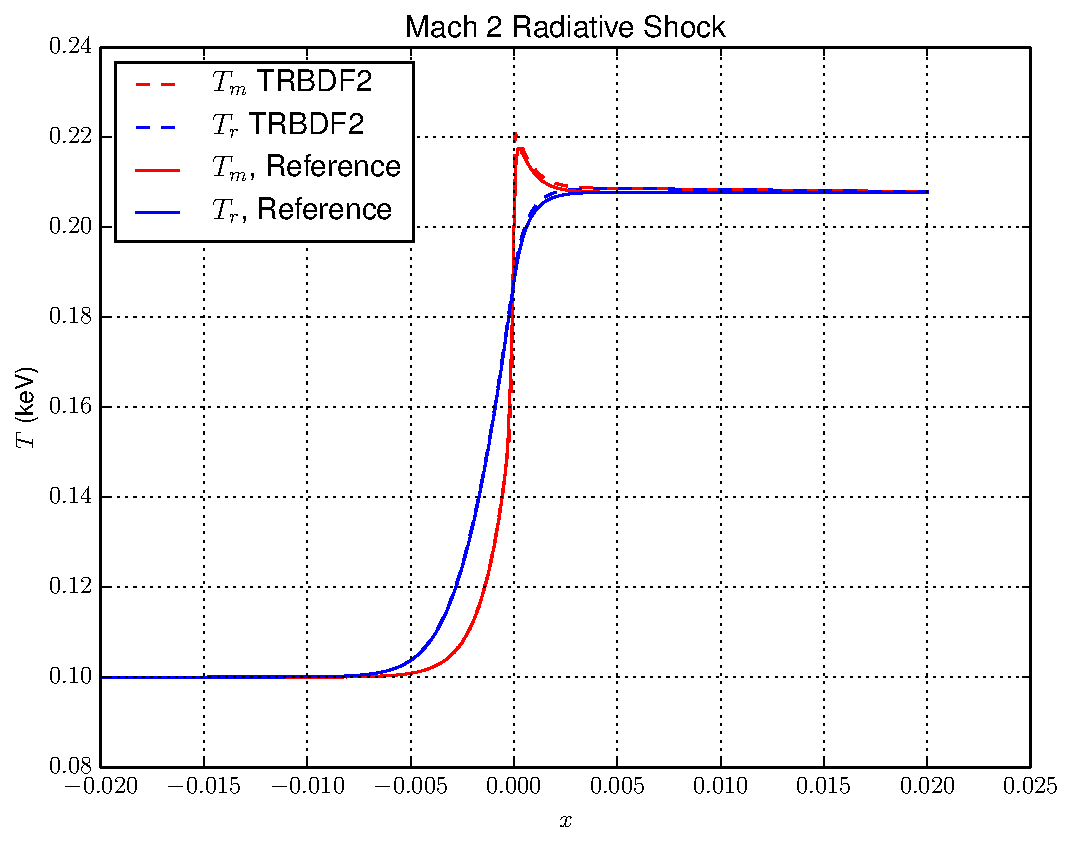
\includegraphics[width=0.9\textwidth]{./figures/mach2_shock.pdf}
\end{center}
\end{frame}

%%%%%%%%%%%%%%%%%%%%%%%%%%%%%%%%%%%%%%%%%%%%%%%%%%%%%%%%%%%%%%%%%%%%%%%%%%%%%%%%%
\begin{frame}
\frametitle{Results}
\framesubtitle{Mach 3 Radiation-Hydrodynamics Shock, 1000 cells}
\begin{center}
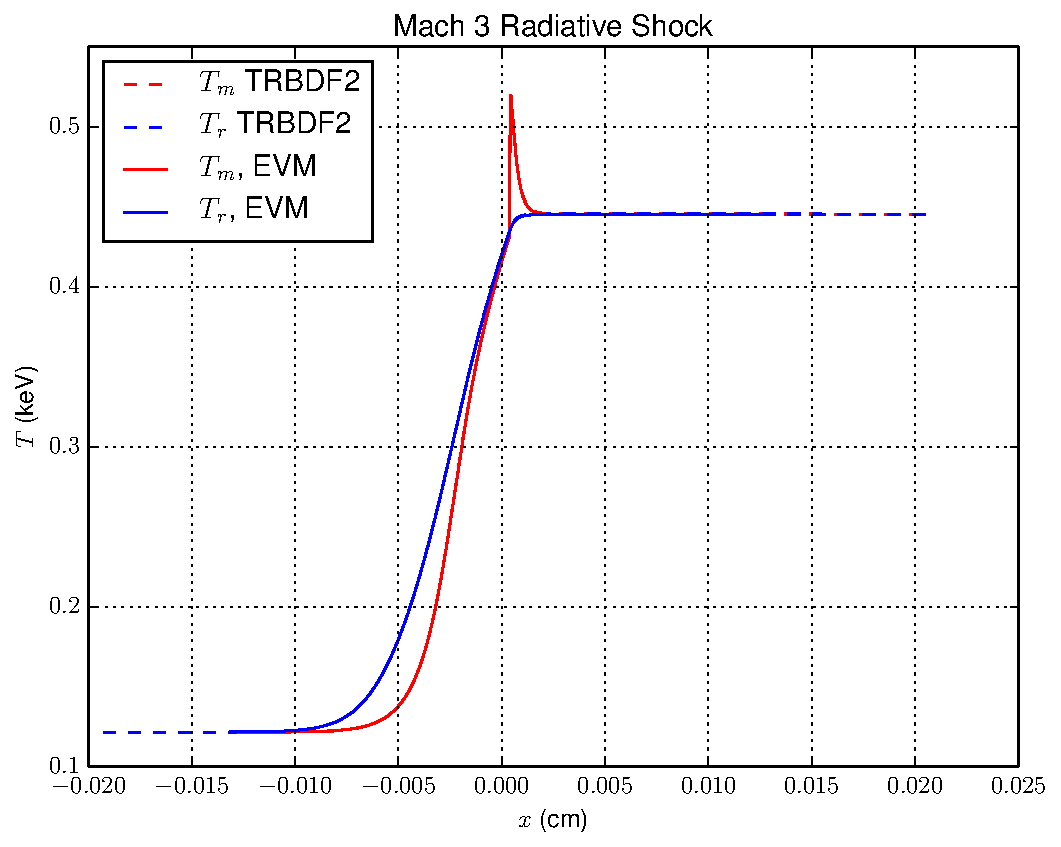
\includegraphics[width=0.9\textwidth]{./figures/mach3_shock.pdf}
\end{center}
\end{frame}

\section{Conclusions and Future Work}

\begin{frame}
    \frametitle{Conclusions}
    
    Demonstrated second order accuracy using manufactured solutions

    Able to obtain accurate solutions in the EDL

    When radiaiton or material motion become insignificant, you get back the
    respective algorithms

\end{frame}




\begin{frame}
    \frametitle{Future Work}
    
    Coupling to a high-order system using hybrid-``S$_2$-like'' equations.

    Exploring slope limiting and EDL, what is going wrong there

    Different way to use internal energy slopes
\end{frame}





\begin{frame}
    \frametitle{Space-Angle LDFE Mesh}
    \noindent
    \fontsize{9.89}{5.0}\selectfont
    \begin{minipage}[t]{0.36\linewidth}
        \centering
        \scalebox{0.8}{
        \begin{tikzpicture}
            \draw (1,1) rectangle (4,4);
            \node[draw,circle,inner sep=1.2 pt,fill] at (2.5,2.5) {};
            \node[above] at (2.5,2.5) {$(x_i,\mu_j)$};
            \draw (1.0,0.4) -- (1.0,0.6) node[below, pos=0.4] {$x_{i-1/2}$};
            \draw (4.0,0.4) -- (4.0,0.6) node[below, pos=0.4] {$x_{i+1/2}$};
            \draw (0.4,1.0) -- (0.6,1.0) node[left, pos=0.4] {$\mu_{j-1/2}$};
            \draw (0.4,4.0) -- (0.6,4.0) node[left, pos=0.4] {$\mu_{j+1/2}$};
            \draw [thick,->] (0.5,0.5) -- (5,0.5) node[anchor=north west] {$x$};
            \draw [thick,->] (0.5,0.5) -- (0.5,5) node[anchor=east] {$\mu$};
        \end{tikzpicture}
    }
    \end{minipage}%
    \begin{minipage}[t]{0.70\linewidth}
        \vspace{-1.6in}
        \hspace{0.5in}
        \begin{itemize}
            \item {\small $\displaystyle \tilde \psi(x,\mu)$} is linear over each
                cell, \colb{preserving} $0^{\text{th}}$ and $1^{\text{st}}$ moment in $x$
                and $\mu$
            \item Use path-length estimators of flux to approximate moments e.g.
            {\small
            \begin{align*}
                \mom{\psi}_{\mu,ij} &= \frac{6}{h_{\mu}^2h_x}
             \iint\limits_\mathcal{D} (\mu-\mu_i) \psi(x,\mu) \d x \d \mu 
        \end{align*}}    
        \end{itemize}
    \end{minipage}
    \pause
    \begin{itemize}
       \item Use standard LD and upwinding to get face terms
    \end{itemize}
\end{frame}



\date{16 October 2015}

\begin{frame}
    \frametitle{{\LARGE\coly{Questions?}}}
    \titlepage \vspace{-0.113in}
\end{frame}

\backupbegin
\appendix

\title{Backup Slides}
\author{}
\date{}

\begin{frame}
    \frametitle{The full equations}
    \begin{itemize}
        \item Material balance equations
\begin{align*}
\pderiv{\rho}{t}+\pderiv{}{x}\fn{\rho u} &= 0 \\
\pderiv{}{t}\fn{\rho u} + \pderiv{}{x}\fn{\rho u^2 + p} &=
\frac{\sigma_t}{c} \F_{0} \\
\pderiv{E}{t} + \pderiv{}{x}\bracket{\fn{E+p}u} &= -\sigma_a c \fn{aT^4 -
\E}+\frac{\sigma_t u}{c} \F_{0} 
\end{align*}
    \item Radiation transport equation, collocated to $\mu=\pm\frac{1}{\sqrt{3}}$
        \begin{equation*}
\frac{1}{c}\pderiv{\psi^\pm}{t} \pm \frac{1}{\sqrt{3}}\pderiv{\psi^\pm}{x} + \sigma_t
\psi^\pm = 
\frac{\sigma_s}{4\pi} c\E + \frac{\sigma_a}{4\pi} acT^4  - \frac{\sigma_t u}{4\pi c}
\F_{0} \pm  
\frac{\sigma_t}{\sqrt{3}\pi}\E u 
\end{equation*}
\end{itemize}
\end{frame}




\backupend
\end{document}

